This report details the calculations of the channel capacity of a Binary Asymmetric Channel where both transition probabilities are independent of each other. A Binary Asymmetric Channel is a channel where a transmitted bit can turn into the other.

\begin{figure}[h!]
    \centering
    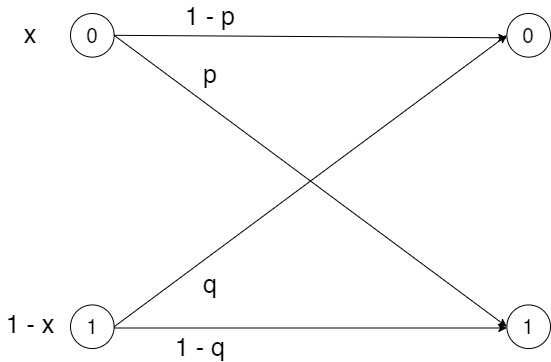
\includegraphics[width = 0.35\textwidth]{images/channel.jpg}
    \caption{Channel Definition}
    \label{fig:channel}
\end{figure}

In this report, it is assumed that the transition probability of a bit from $0$ to $1$ is $p$ and from $1$ to $0$ is $q$. Also, the probability of the inputs bits themselves are $x$ and $(1-x)$. We find the optimum input bit distribution for any channel characteristic i.e., p and q and thereby find the maximum allowable capacity for an arbitrarily slow error that asymptotically goes to $0$.

In section \ref{derive}, the capacity values are calculated theoretically. Section \ref{implement} shows the MATLAB implementation to verify the derivations and section \ref{results} documents the results. Finally, section \ref{discuss} looks the interpretation of the results and provides a subjective opinion on the performance of the channels.

From this point on, the Binary Asymmetric Channel where only one transition is possible is referred to as Z Channel and when two transitions are possible, the channel is referred to as Binary Asymmetric Channel or BSC. The Binary Symmetric Channel is also referred to as BAC.